%%
%% $Id: AstroTaverna.tex
%%
%%

%% Use the option review to obtain double line spacing
%% \documentclass[authoryear,preprint,review,12pt]{elsarticle}

%% Use the options 1p,twocolumn; 3p; 3p,twocolumn; 5p; or 5p,twocolumn
%% for a journal layout:
%% \documentclass[final,authoryear,1p,times]{elsarticle}
%% \documentclass[final,authoryear,1p,times,twocolumn]{elsarticle}
%% \documentclass[final,authoryear,3p,times]{elsarticle}
%% \documentclass[final,authoryear,3p,times,twocolumn]{elsarticle}
%% \documentclass[final,authoryear,5p,times]{elsarticle}
\documentclass[final,authoryear,5p,times,twocolumn]{elsarticle}

%%
\usepackage{color}
%% if you use PostScript figures in your article
%% use the graphics package for simple commands
\usepackage{graphics}
%% or use the graphicx package for more complicated commands
%%\usepackage{graphicx}
%% or use the epsfig package if you prefer to use the old commands
%% \usepackage{epsfig}

%% The amssymb package provides various useful mathematical symbols
%% \usepackage{amssymb}
%% The amsthm package provides extended theorem environments
%% \usepackage{amsthm}

%% The lineno packages adds line numbers. Start line numbering with
%% \begin{linenumbers}, end it with \end{linenumbers}. Or switch it on
%% for the whole article with \linenumbers after \end{frontmatter}.
%% \usepackage{lineno}

%%%%%%%%%%%%%%%%%%%%%%%%%%%%%%%%%%%%%%%%
\usepackage{txfonts}
%%%%%%%%%%%%%%%%%%%%%%%%%%%%%%%%%%%%%%%%
\usepackage[breaklinks=true]{hyperref}

%% natbib.sty is loaded by default. However, natbib options can be
%% provided with \biboptions{...} command. Following options are
%% valid:

%%   round  -  round parentheses are used (default)
%%   square -  square brackets are used   [option]
%%   curly  -  curly braces are used      {option}
%%   angle  -  angle brackets are used    <option>
%%   semicolon  -  multiple citations separated by semi-colon (default)
%%   colon  - same as semicolon, an earlier confusion
%%   comma  -  separated by comma
%%   authoryear - selects author-year citations (default)
%%   numbers-  selects numerical citations
%%   super  -  numerical citations as superscripts
%%   sort   -  sorts multiple citations according to order in ref. list
%%   sort&compress   -  like sort, but also compresses numerical citations
%%   compress - compresses without sorting
%%   longnamesfirst  -  makes first citation full author list
%%
%% \biboptions{longnamesfirst,comma}

\journal{Astronomy and Computing}

\newcommand{\urlsamefont}[1]{\urlstyle{same}\url{#1}}
\newcommand{\hrefnote}[2]{\href{#1}{#2}\footnote{\urlsamefont{#1}}}
\newcommand*\acknowledgements{\tiny}

\begin{document}

\begin{frontmatter}

%% Title, authors and addresses

%% use the tnoteref command within \title for footnotes;
%% use the tnotetext command for the associated footnote;
%% use the fnref command within \author or \address for footnotes;
%% use the fntext command for the associated footnote;
%% use the corref command within \author for corresponding author footnotes;
%% use the cortext command for the associated footnote;
%% use the ead command for the email address,
%% and the form \ead[url] for the home page:
%%
%% \title{Title\tnoteref{label1}}
%% \tnotetext[label1]{}
%% \author{Name\corref{cor1}\fnref{label2}}
%% \ead{email address}
%% \ead[url]{home page}
%% \fntext[label2]{}
%% \cortext[cor1]{}
%% \address{Address\fnref{label3}}
%% \fntext[label3]{}

\title{AstroTaverna - Building workflows with Virtual Observatory services}

%% use optional labels to link authors explicitly to addresses:
%% \author[label1,label2]{<author name>}
%% \address[label1]{<address>}
%% \address[label2]{<address>}

\author[IAA]{Ruiz, J.E.\corref{cor1}}
\ead{jer@iaa.es}
\cortext[jer]{\textit{Phone number: +34 958 230 618}}

\author[IAA]{Garrido, J.\corref{cor1}}
\ead{jgarrido@iaa.es}
\cortext[cor1]{\textit{Corresponding author}}

\author[IAA]{Santander-Vela, J.D.}
\ead{jdsant@iaa.es}
\author[IAA]{S\'anchez-Exp\'osito, S.}
\ead{sse@iaa.es}
\author[IAA]{Verdes-Montenegro, L.}
\ead{lourdes@iaa.es}

\address[IAA]{Instituto de Astrof\'isica de Andaluc\'ia - CSIC \\Glorieta de la Astronom\'ia s/n, 18008 Granada, Spain}


\begin{abstract}
%% Text of abstract
Despite the long tradition of publishing digital datasets in Astronomy, and the existence of a rich network of services providing astronomical datasets in standardized interoperable formats through the Virtual Observatory (VO), there has been little use of scientific workflow technologies in this field. In this paper we present AstroTaverna, a plugin that we have developed for the Taverna Workbench scientific workflow management system. It integrates existing VO web services as first-class building blocks in Taverna workflows, allowing the digital capture of otherwise lost procedural steps manually performed in e.g. GUI tools, providing reproducibility and re-use. It improves the readability of digital VO recipes with a comprehensive view of the entire automated execution process, complementing the scarce narratives produced in the classic documentation practices, transforming them into \textit{living tutorials} for an efficient use of the VO infrastructure. The plugin also adds astronomical data manipulation and transformation tools based on the STIL Tool Set and the integration of Aladin VO software, as well as interactive connectivity with SAMP-compliant astronomy tools. 
\end{abstract}

\begin{keyword}
%% keywords here, in the form: keyword \sep keyword
Virtual observatories; Astroinformatics; methods: data analysis; methods: miscellaneous; astronomical databases: miscellaneous; e-Science; Scientific workflows
%% MSC codes here, in the form: \MSC code \sep code
%% or \MSC[2008] code \sep code (2000 is the default)
\end{keyword}

\end{frontmatter}

%% main text
\section{Introduction}
\label{Introduction}

In recent decades Astronomy has witnessed the development of instrumentation performing observations of the sky across the full range of the electromagnetic spectrum. The advent of automated survey facilities has dramatically increased the number of archival datasets and transformed the approach to deal with key science topics, now potentially benefitting from seamless access to interoperable multi-wavelength data. The \hrefnote{http://www.ivoa.net/}{International Virtual  Observatory Alliance} (IVOA) was created with the goal of developing standards and their implementations for exchange of astronomical data, and maintaining registries of data repositories and services. The Virtual Observatory (VO) provides a way to transparently access and extract scientific knowledge from multiple archives of astronomical data, enabling standardised services discovery and access to interoperable data.  The VO consists of a network of web-distributed data services which provides free access to astronomical catalogues, images and spectrum data, that combined with tools for local visualization and analysis (VO Apps) allow astronomers to graphically explore the different data sets, all following IVOA recommendations.

VO Apps are any kind of local software able to access the elements of the VO data network, following IVOA protocols, and sometimes permitting discovery of services available in the VO Registry~\citep{Benson2009} in order to provide the users with their datasets of  interest. Current VO Apps are mainly of two-kinds: general purpose tools for accessing a particular kind of data (catalogues, images, or spectra); and custom-built programs and scripts created by astronomers in order to perform their scientific research. Both kinds of tools are typically used together for a science use case, with the user performing each step with different tools. This means that, in order to register the fully procedural protocol so it can be reproduced and possibly encapsulated in a more complex process, the user needs to manually capture the dependencies between steps, which is currently accomplished by writing scripts driving the execution of other tools or scripts.

Digital scientific workflows~\citep{Gil2007, Gil2008} allow capturing the actions performed in accessing distributed data, their aggregation and analysis using third-party services, as they identify and record the provenance leading to the final obtained results. They facilitate the means to come up with \emph{in silico} reproducible research, that can be shared, executed or even modified by other scientists in the community. Workflows provide a comprehensive explicit exploratory view of the scientific protocol, while being at the same time the precise and well-codified description needed by the underlying engine to execute the whole multi-step process. Unlike traditional pipelines, which tend to produce scientifically exploitable data, most of the scientific workflows are aimed at producing scientific insight.

\hrefnote{http://www.taverna.org.uk/}{Taverna}~\citep{Wolstencroft01072013} is an open source, domain-independent scientific workflow management system that has grown popular in fields like bioinformatics, chemistry, text mining, and image analysis. It is a suite of tools including Taverna Workbench, a desktop client application used to graphically design, create, edit and execute scientific workflows. Taverna workflows can also be executed on the command line or on an installation of the Taverna Server.

The Taverna Workbench is specially designed to combine distributed web services and local tools into complex workflows, the basics building blocks of VO-services-based scientific workflows. It also integrates workflow discovery and publishing through dedicated UI for access to the \hrefnote{http://www.myexperiment.org/}{myExperiment}~\citep{Goble2010} public digital library of workflows. Moreover, its plugin architecture allows loose integration and open-source developments of plugins, decoupled from core developments of Taverna Workbench.

In this paper we present AstroTaverna, a plugin that simplifies the use of VO services from within the Taverna Workbench 2.x, by providing VO-service discovery facilities, and building blocks for VO data access and manipulation. AstroTaverna provides astronomers with the means to compose scientific workflows of standardized VO-services, together with existing local and distributed tools. In Sect.~\ref{RelatedWork} we provide a very brief overview of workflow related initiatives we are aware of in Astronomy. In Sect.~\ref{Opening} we describe the Taverna Workbench and the main VO architectural elements taken into account in the implementation of AstroTaverna. In Sect.~\ref{Design} we provide a description of the functional drivers that led the developments of AstroTaverna as well as its main features, illustrating them all with an example use case. In Sect.~\ref{ResultsAndDiscussion} we provide a discussion on the impact of the use of workflows in the community in the context of the results issued from AstroTaverna developments, as well as future plans for its dissemination and improvements. Finally, in Sect.~\ref{Conclusions} the main conclusions of the exposed work are presented. 

\section{Related work}
\label{RelatedWork}

There have been several attempts of bringing workflow technologies to the astronomy field, and in particular with the Taverna workflow system. The \hrefnote{http://www.eso.org/sci/software/sampo/}{ESO Sampo} project performed a feasibility study for the integration of the ESO pipeline processing tools with the Taverna 1 workflow engine. The study gave birth to the \hrefnote{http://www.eso.org/sci/software/sampo/reflex/}{ESO Reflex} subproject~\citep{Hook2009}, using the Kepler engine~\citep{Altintas2004} instead. Recently, the \hrefnote{http://www.helio-vo.eu/}{HELIO} project~\citep{Bentley2013} has successfully used the Taverna 2 workflow engine, by creating heliophysics-specific services that provide support for their scientific use cases in a Service-Oriented Architecture. 

Other workflow related software and initiatives are the \hrefnote{http://www.trianacode.org/}{Triana}~\citep{Taylor2007} and \hrefnote{http://pegasus.isi.edu/}{Pegasus}~\citep{Deelman:2005:PFM:1239649.1239653} workflow environments, as well as workflow implementations of \hrefnote{http://montage.ipac.caltech.edu/}{Montage} image mosaicing software. On a different angle, projects like \hrefnote{http://www.astro-wise.org/}{Astro-WISE}, IceCore~\citep{Maisala2012} and \hrefnote{http://www.cyberska.org/}{CyberSKA} ~\citep{Kiddle2011} have provided web interfaces for the building and execution of workflows based on proprietary services running in their server infrastructure. The \hrefnote{http://www.erflow.eu/}{ER-Flow} project aims to create a workflow user community across Europe in different fields of scientific research. It provides support for communities working in Astronomy and Heliophysics, with workflows developed in a variety of workflow systems, workflow engines and workflow languages, that are later implemented in their own cyber-infrastructure through the \hrefnote{https://shiwa-portal2.cpc.wmin.ac.uk/liferay-portal-6.1.0/}{SHIWA Portal}.

In general, workflow related approaches in Astronomy deal with very specialized proprietary data reduction pipelines, which tend to produce scientifically exploitable data, still distant from the \textit{ready for publish} scientific insight. There has been little effort, to our knowledge, to integrate Virtual Observatory publicly accessible data and services into the workflows working methodology. In this context, the VO-France Workflow working group~\citep{Schaaff2008} aims to provide use cases to implement them as workflows with VO enabled workflow tools, and we may also find JLOW plugin -- a graphical tool that allows the design and execution of workflows based on Aladin ~\citep{Bonnarel2000} tasks available at the \hrefnote{http://aladin.u-strasbg.fr/java/nph-aladin.pl?frame=plugRep}{Aladin plugin repository}. 

The \hrefnote{http://www.astrogrid.org/}{AstroGrid} project undertook the development of tools to design and execute VO-services-based scientific workflows. AstroGrid created a modified version of the Taverna 1 workflow engine~\citep{Benson2009, Walton2010} which integrated VO Apps in the source code of the tool. Unfortunately the final result was not publicly relased, though the code has been re-used in the development of a plugin for Taverna 2 workflow engine in the frame of the \hrefnote{http://www.vamdc.eu/}{VAMDC}~\citep{Walton2011} project. This plugin allows the building and execution of workflows based on very specific services running in the project infrastructure, its use remaining again inside the scope of its own project. 

\section{Opening Taverna to the Virtual Observatory}
\label{Opening}

\subsection{The Taverna Workbench}
\label{TavernaWorkbench}

The Taverna Workbench allows scientists to assemble data and analytical services in a graphical workflow, connecting tools by specifying the desired flow of data (inputs and outputs) rather than a fixed execution order. It provides the scientist with a tool for designing and executing workflows, playfully combining local and external processes with data, as well as with support for service and workflow discovery. Such workflows typically combine a wide range of third-party tools, ranging from RESTful and SOAP web services, SQL databases and grid infrastructures, to local command line tools and embedded scripts. They can then be processed on the Taverna Workbench (desktop application), using the Taverna Command Line, or on installations of the Taverna Server (remote location).

Taverna Workbench additionally offers tools for browsing provenance, and inspect workflow runs, allowing the exploration of intermediate results from past invocations. Execution of workflows is optimized because of its intra-processing data parallelism, users may fine-tune the behavior of processes as well as define error-handling tactics, and follow the progress of the execution of the workflow through its dependencies in an interactive monitor, browsing outputs and intermediate values as they are produced.

The \textit{executable graph} provided by a workflow does not guarantee on its own a full understanding of the scientific method, neither reusability nor reproducibility~\citep{WfRO:SePublica2012}. This understanding is specially needed in collaborative science, where sharing executable recipes is vital to avoid duplication of effort and reinvention, as well as to assess soundness of the scientific methodology. To overcome these issues, additional information may be needed to better document the process. Taverna Workbench allows the workflow designer to add free-text descriptions on the elements of the workflow, which can be seen as complementary information about the science involved, assumptions made, hypothesis to be proven, the configuration of the execution environment, caveats and still unresolved issues, etc.

Although these are already major advantages over manual analysis methods and scripting, Taverna Workbench also supports the integration of local scripts and tools as workflow components. These processes are executed as if they were launched at the terminal command line, allowing the full orchestration of local and external resources in a single workflow, where the entire procedural protocol is captured and possibly documented. 

\subsection{The Virtual Observatory architecture}
\label{VirtualObservatory}

The Virtual Observatory infrastructure provides the community electronic access to numerous sources of information.  Users consume transparently the VO-technologies by using astronomy VO-compliant local software \textendash VO App in Fig.~\ref{fig:VOArch}\textendash\ or using a web browser to access a VO-enabled web portal. In order to access either locally archived or remote files, they must only be aware of the different applications of their interest, and that there exist interoperable image, spectra, and catalogue servers, transparently accessed from their toolset. They must also be aware that some applications can send messages and data between them, sending for instance data to be analysed to some applications, and sending the received results to other applications for plotting. 

All the elements of the architecture outside the local user environment \textendash dotted cloud in Fig.~\ref{fig:VOArch}\textendash\ are indispensable for the operation of the VO, but are completely transparent to the user. It is very common that VO App users deal simultaneously with local and remote data by invoking VO services encapsulated in the VO Apps. These services are known by the applications since they are indexed in registry servers (VO Registry).

VO services are either SOAP (for the access to the VO Registry), or RESTful (for data access protocols) web services. Taverna Workbench provides tools for directly accessing this kind of services, but that means that discovery of these services is left to the user (while service discovery is integral for VO Apps), together with a certain knowledge of web services and the parameters required by each data access. AstroTaverna has been designed to provide the means for easy discovery and query of VO data access services. In addition, functionality for the manipulation and visualization of VOTables has also been added in order to make VO services first-class building blocks for Taverna workflows.

\begin{figure}[tb]
\centering
\resizebox{\hsize}{!}{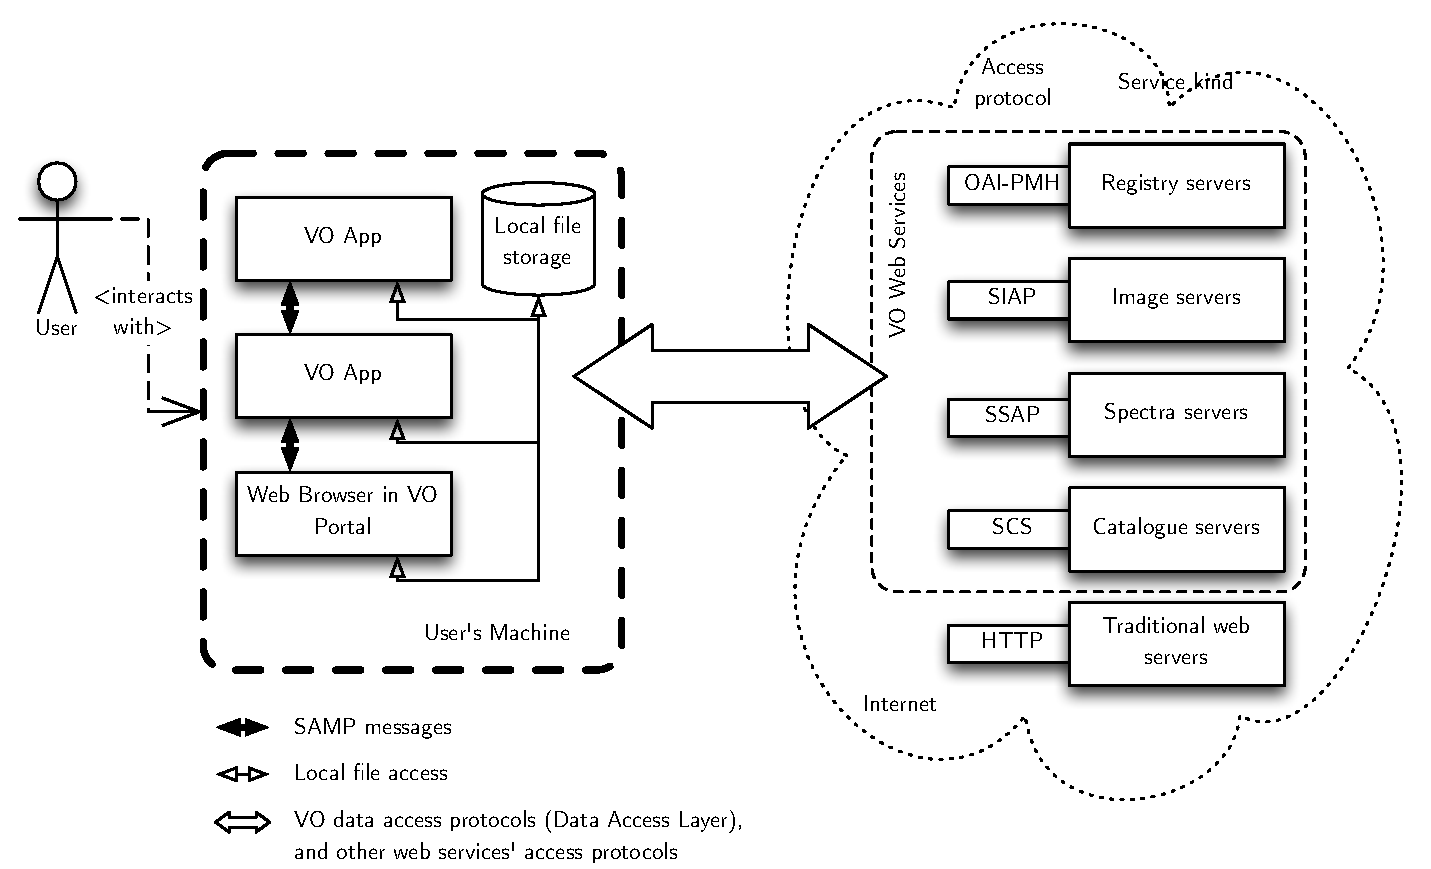
\includegraphics{VOArch.pdf}} 
\caption{Virtual Observatory usage and architecture.}
\label{fig:VOArch}
\end{figure}

The main VO architectural elements that have been implemented in AstroTaverna are:

\begin{itemize}
\item The VO Registry: based on the Open Archives Initiative resource metadata~\citep{2002OAI-PMH},  it provides services registered in the form of VO Resources ~\citep{Hanisch2007}. Specializations of the VO Resource exist for identifying image data services~\citep[Simple Image Access Protocol;][]{Tody2009}, spectral data services~\citep[Simple Spectral Access Protocol;][]{Tody2012}, positional-search table services~\citep[ConeSearch Protocol;][]{Williams2008}, and tabular complex searches~\citep[Tabular Access Protocol;][]{Dowler2010}. Each entry contains metadata identifying the curators and publishers of the data, service type, service-type specific descriptions, or the URL for the services’ entry points. 

\item VO Services: the VO data access services implemented in AstroTaverna are those compliant with IVOA standards for the more used \textit{simple data access protocols}\footnote{http://www.ivoa.net/documents/} (ConeSearch Protocol, Simple Image Access Protocol, Simple Spectral Access Protocol). These services accept parameterized inputs encoded in one URI that is used as entry point to query the services. Data returned are always in VOTable format. Science data are embedded in the VOTable, or linked from data access fields.

\item VO Apps: TOPCAT~\citep{Taylor2011} and Aladin are VO Apps widely used in the VO community providing enhanced capabilities for tabular data management and inspection, as well as simple tasks for multi-wavelength image visualization, analysis and comparison. Some of these capabilities may be fully integrated in Taverna Workbench as local services performing very specific tasks based on STIL API and STILTS Java framework~\citep{Taylor2006,STILTS2011}, or executing scripts and macros in the case of Aladin. Integrating STILTS in AstroTaverna also grants direct access to most common functionalities provided by this library. Extended functionalities may be accessed making use of scripts through Taverna Beanshells. Finally, the SAMP~\citep[Simple Application Messaging Protocol;][]{Taylor2012} messaging protocol enables data exchange and communication among local tools, allowing new born tools like AstroTaverna plugin to send intermediate data and/or results to locally installed VO Apps for enhanced data inspection.
\end{itemize}

\section{AstroTaverna design}
\label{Design}

\subsection{Functional drivers}
\label{FunctionalDrivers}

The AstroTaverna plugin targets users with no special technical knowledge of the underlying applications involved in the workflow execution process. It has been conceived to be easy to install and allow users to design, create and fully understand workflows without commissioning specialists or hiring software engineers. It provides the users with the means to design, build and execute VO-services-based workflows through the Taverna Workbench.

AstroTaverna aims to provide universal access to tabular representations of data issued by most of VO services recorded in the VO Registry. It supports open science and open data access. In the VO context, standardized workflows could be helpful to gather and aggregate data from distributed datasets, in order to engage multi-epoch and multi-band comparative astrophysics. The vision of a workflow as the orchestration of tools and tasks running either locally or externally may be greatly improved if we consider the VO as a rich infrastructure of web services and data, where VO services may be used as components for web-services-based workflows. 

The focus of AstroTaverna lies in enhancing the documentation of the scientific process, where the transparency of the method is exposed in an interactive monitor showing the progress of the execution of the workflow. The automation of the process is a nice-to-have feature, but already accomplished by many scientists through different scripting languages and environments with no help of workflow tools. The main goal of AstroTaverna is improving readability and enabling reproducibility of digital VO recipes, capturing and registering provenance information of the whole experimental protocol otherwise lost in procedural steps manually performed in GUIs of VO Apps. 

The main functional drivers to be addressed by the AstroTaverna plugin are:
\begin{itemize}
\item
\textit{Data discovery, gathering and aggregation.}\\
AstroTaverna aims to be an open window to public astronomical data and services. We take advantage of the infrastructure of interoperable data provided by the VO in order to build, for a sample of objects, tabular representations of their properties extracted from different archives. These tables may be rebuilt at any moment from the re-execution of the workflow, hence providing up-to-date information when refreshed.
\item
\textit{Data manipulation, filtering and cross matching.}\\
The interoperable VOTable~\citep{Ochsenbein2009} data format provided by the VO allows efficient manipulation and combination of datasets coming from different archives. Tabular data should be handled along the workflow with no need to address major format conversion issues, but focusing on basic operations for data management (e.g. cross matching, filtering, table merging and concatenation, row/column extraction and addition, etc.) in order to shape and rebuild information based on very specific needs.
\item
\textit{Data transformation.}\\
We have considered allowing actions on datasets going beyond data massage and manipulation, hence altering their values. Operations like transformation of sky coordinates and among reference systems, resolution of source names into coordinates, addition of new data based on existing ones, etc. are commonly used when working with tabular data of astronomical objects. More complex data transformations could be possible by adding small code snippets of scripts (e.g. Python, bash, etc.) or local command line software.
\item
\textit{VO software integration and data inspection.}\\
In order to benefit from widely used and well known functionalities of established VO Apps Topcat and Aladin, we decided to integrate some of their specific tasks. Moreover, in order to achieve a full understanding of final and intermediate data a proper rendering of the VOTable format was needed. Sharing these data with local VO Apps in a seamless way would allow each user to individually perform enhanced data inspection at any moment, which does not affect the reproducibility of the workflow and the final results.
\end{itemize}

\subsection{Data discovery, gathering and aggregation}
\label{DataDiscovery}

AstroTaverna provides support for discovery of VO data access services, with the addition of a new \textit{VO Service} tab to the perspectives menu located on the top of Taverna Workbench window. This perspective, as seen in Fig.~\ref{fig:VODiscovery}, allows users to discover, browse, inspect and add VO services to workflows in the process of design. Users may select the VO Registry URL endpoint where they would like to perform the search of VO services. This search is based on keywords entered on a free-text box as well as on the specific service type chosen: Cone Search (positionally-indexed tabular data), SSA (positionally-indexed spectra) and SIA (positionally-indexed images). The list of VO services found is then presented as a tabular list with columns for the service \textit{Short name, Title, Subjects, Identifier} and \textit{Publisher}. The query interface is very similar to the one proposed in the widely used TOPCAT VO application. 

When one of the services is selected among the list, a more detailed description is displayed on the right panel, with metadata extracted from the VO Registry. The user may, at this point, decide to use the service in the design process of a workflow pressing the \textit{Add to workflow} button. This action opens a window allowing a more detailed definition of the specific artifact that will be created associated to this service on the \emph{Design} perspective of Taverna Workbench. The AstroTaverna plugin provides the user with the possibility to create these artifacts on the workflow design with fixed parameter values entered on this form. Alternatively, the parameter can be supplied from a previous step in the workflow. Optional, service-specific query parameters can similarly be enabled as inputs or given a fixed value. VO services may also be added directly into the \emph{Design} perspective in drag-and-drop actions from the services panel. In this case the user needs to know the exact URL of the added RESTful web service, as the VO Registry discovery process is not involved. This mechanism is useful while services are under development or not yet registered in the registry.

\begin{figure}[tb]
\centering 
\resizebox{\hsize}{!}{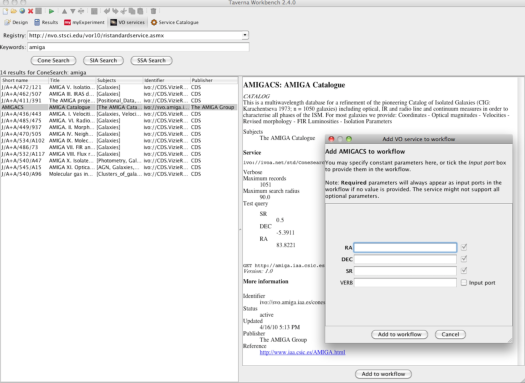
\includegraphics{VODiscovery.pdf}}
\caption{AstroTaverna user interface for discovery of VO data access services. The list of services found is displayed on the left panel, the description and input parameters of a selected service is shown on the right panel and floating window.}
\label{fig:VODiscovery}
\end{figure}

\subsection{Data manipulation, filtering and cross matching}
\label{DataManipulation}

Given that the data returned by VO services are interoperable VOTables, there is a need for tools allowing actions for efficiently manipulating tabular data, as well as tools providing format conversion between VOTable format and others widely used tabular formats in astronomy research (e.g. FITS, CSV, TST, ASCII, HTML, etc.). Furthermore, spatial table cross matching (finding rows in other tables which might be near a given position, with a prescribed tolerance) and table joins on common keys are also common actions that need to be covered in data manipulation basic capabilities.

AstroTaverna provides a collection of built-in data manipulation services, listed as \hrefnote{http://amiga.iaa.es/p/312-astrotools.htm}{\textit{Astro tools}} within Taverna's services panel.

\begin{itemize}
\item \textit{VOTable format conversion}
\item \textit{Concatenate two VOTables}
\item \textit{Concatenate a list of VOTables}
\item \textit{Join two VOTables}
\item \textit{Add common fields to a VOTable}
\item \textit{Crossmatch two VOTables}
\item \textit{Select columns from a VOTable}
\item \textit{Extract column from a VOTable as a list}
\item \textit{Select rows from a VOTable}
\end{itemize}

These services, shown in Fig.~\ref{fig:design}, can be dragged and added to the workflow diagram in the central design panel. They include table row filtering by boolean algebraic expressions on field values and column subsets.  The expressions for row filtering and column selection follow the STILTS syntax\footnote{\urlsamefont{http://www.star.bristol.ac.uk/~mbt/stilts/sun256/jel.html}} \footnote{\urlsamefont{http://www.star.bristol.ac.uk/~mbt/stilts/sun256/colid-list.html}}.

\begin{figure}[tb]
\centering 
\resizebox{\hsize}{!}{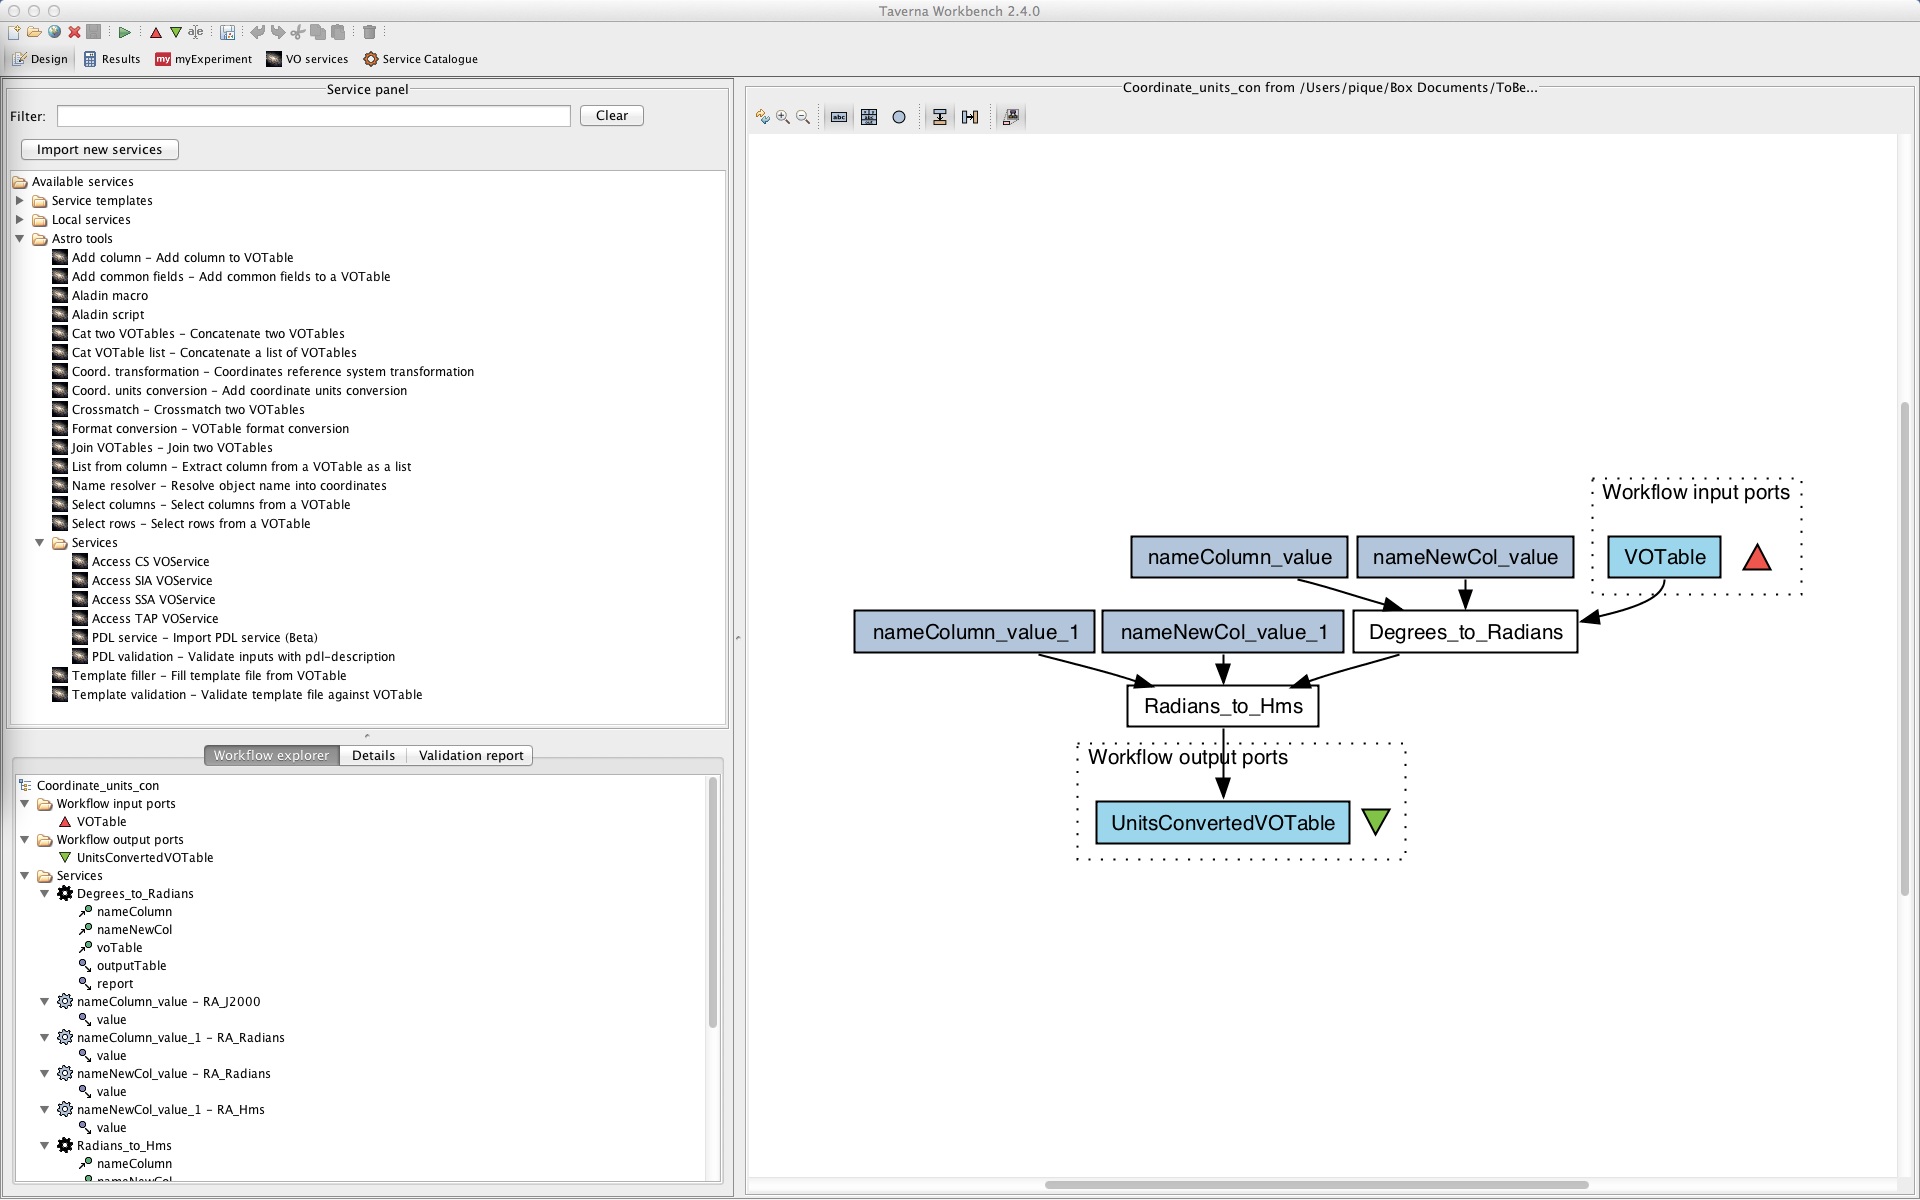
\includegraphics{design.png}}
\caption{Workflow design in Taverna Workbench, showing \textit{Astro tools} services on the upper left panel and a workflow for coordinate unit conversion on the \emph{Design} perspective. Adapted from \url{http://www.myexperiment.org/workflows/3515}}
% \caption{Workflow design in Taverna Workbench, showing \textit{Astro tools} services and a workflow for coordinate unit conversion. Adapted from myExperiment workflow \#3515, \urlsamefont{http://www.myexperiment.org/workflows/3515}.}
\label{fig:design}
\end{figure}

\subsection{Data transformation}
\label{DataTransformation}

On the same basis, AstroTaverna also provides a collection of services for transformation of VOTable data. These include the addition of columns based on calculations and/or basic combination of existing ones, following algebraic expressions, transformation of sky coordinates and between different reference systems (e.g. equatorial, ecliptic, galactic, and others), resolution of astronomical object names into equatorial (Right Ascension, Declination) coordinates using the \hrefnote{http://cdsweb.u-strasbg.fr/doc/sesame.htx}{Sesame service}, as well as the conversion of coordinates between different units. These are the following:

\begin{itemize}
\item \textit{Add column to a VOTable}
\item \textit{Add coordinate units conversion}
\item \textit{Resolve object name into coordinates} 
\item \textit{Coordinates reference system transformation}
\end{itemize}

Other two services have been added related with the creation and validation of text files using templates. These templates may be provided in the workflow, and used together with information extracted from VOTables in order to create local files \textit{on-the-fly} (e.g. software configuration files or input data files in a given specific format).

\begin{itemize}
\item \textit{Fill template file from VOTable}
\item \textit{Validate template file against VOTable}
\end{itemize}

More complex data transformations may be possible using the \textit{Tool} service provided by Taverna Workbench to locally execute specific command line software or OS commands and small script files. This is especially useful when adding existing snippets of scripts (e.g. Python, bash, etc.) commonly used in astronomy research.  

\subsection{VO software integration and data inspection}
\label{VOApps}

Proper rendering of VOTables is needed in order to allow inspection of intermediate and final values issued from the data workflow. AstroTaverna provides the possibility to display the XML-formatted VOTables in the \emph{Results} perspective, together with their field’s metadata, in a spreadsheet-like form, as shown in Fig.~\ref{fig:WfExec}. It also implements the SAMP message exchange protocol, allowing the user to send VOTable data to local SAMP-enabled software. SAMP connects AstroTaverna workflows with other VO Apps, giving the user the possibility to perform post-workflow data inspection and analysis using more specific local software.

The Aladin VO App is bundled into the AstroTaverna plugin, which allows the user to execute Aladin macros and scripts using data extracted from VOTables provided by VO services. The Aladin services may be configured with the GUI option enabled, which triggers the visual automated execution of actions on Aladin VO App during the process of workflow execution. The specific output of these Aladin services is a VOTable containing the path and filenames of the final images and planes saved on the local disk during the executions of macros and/or scripts, according to the commands present on the scripts.

\subsection{Example use case}
\label{Usecase}

\begin{figure*}[tb]
\centering 
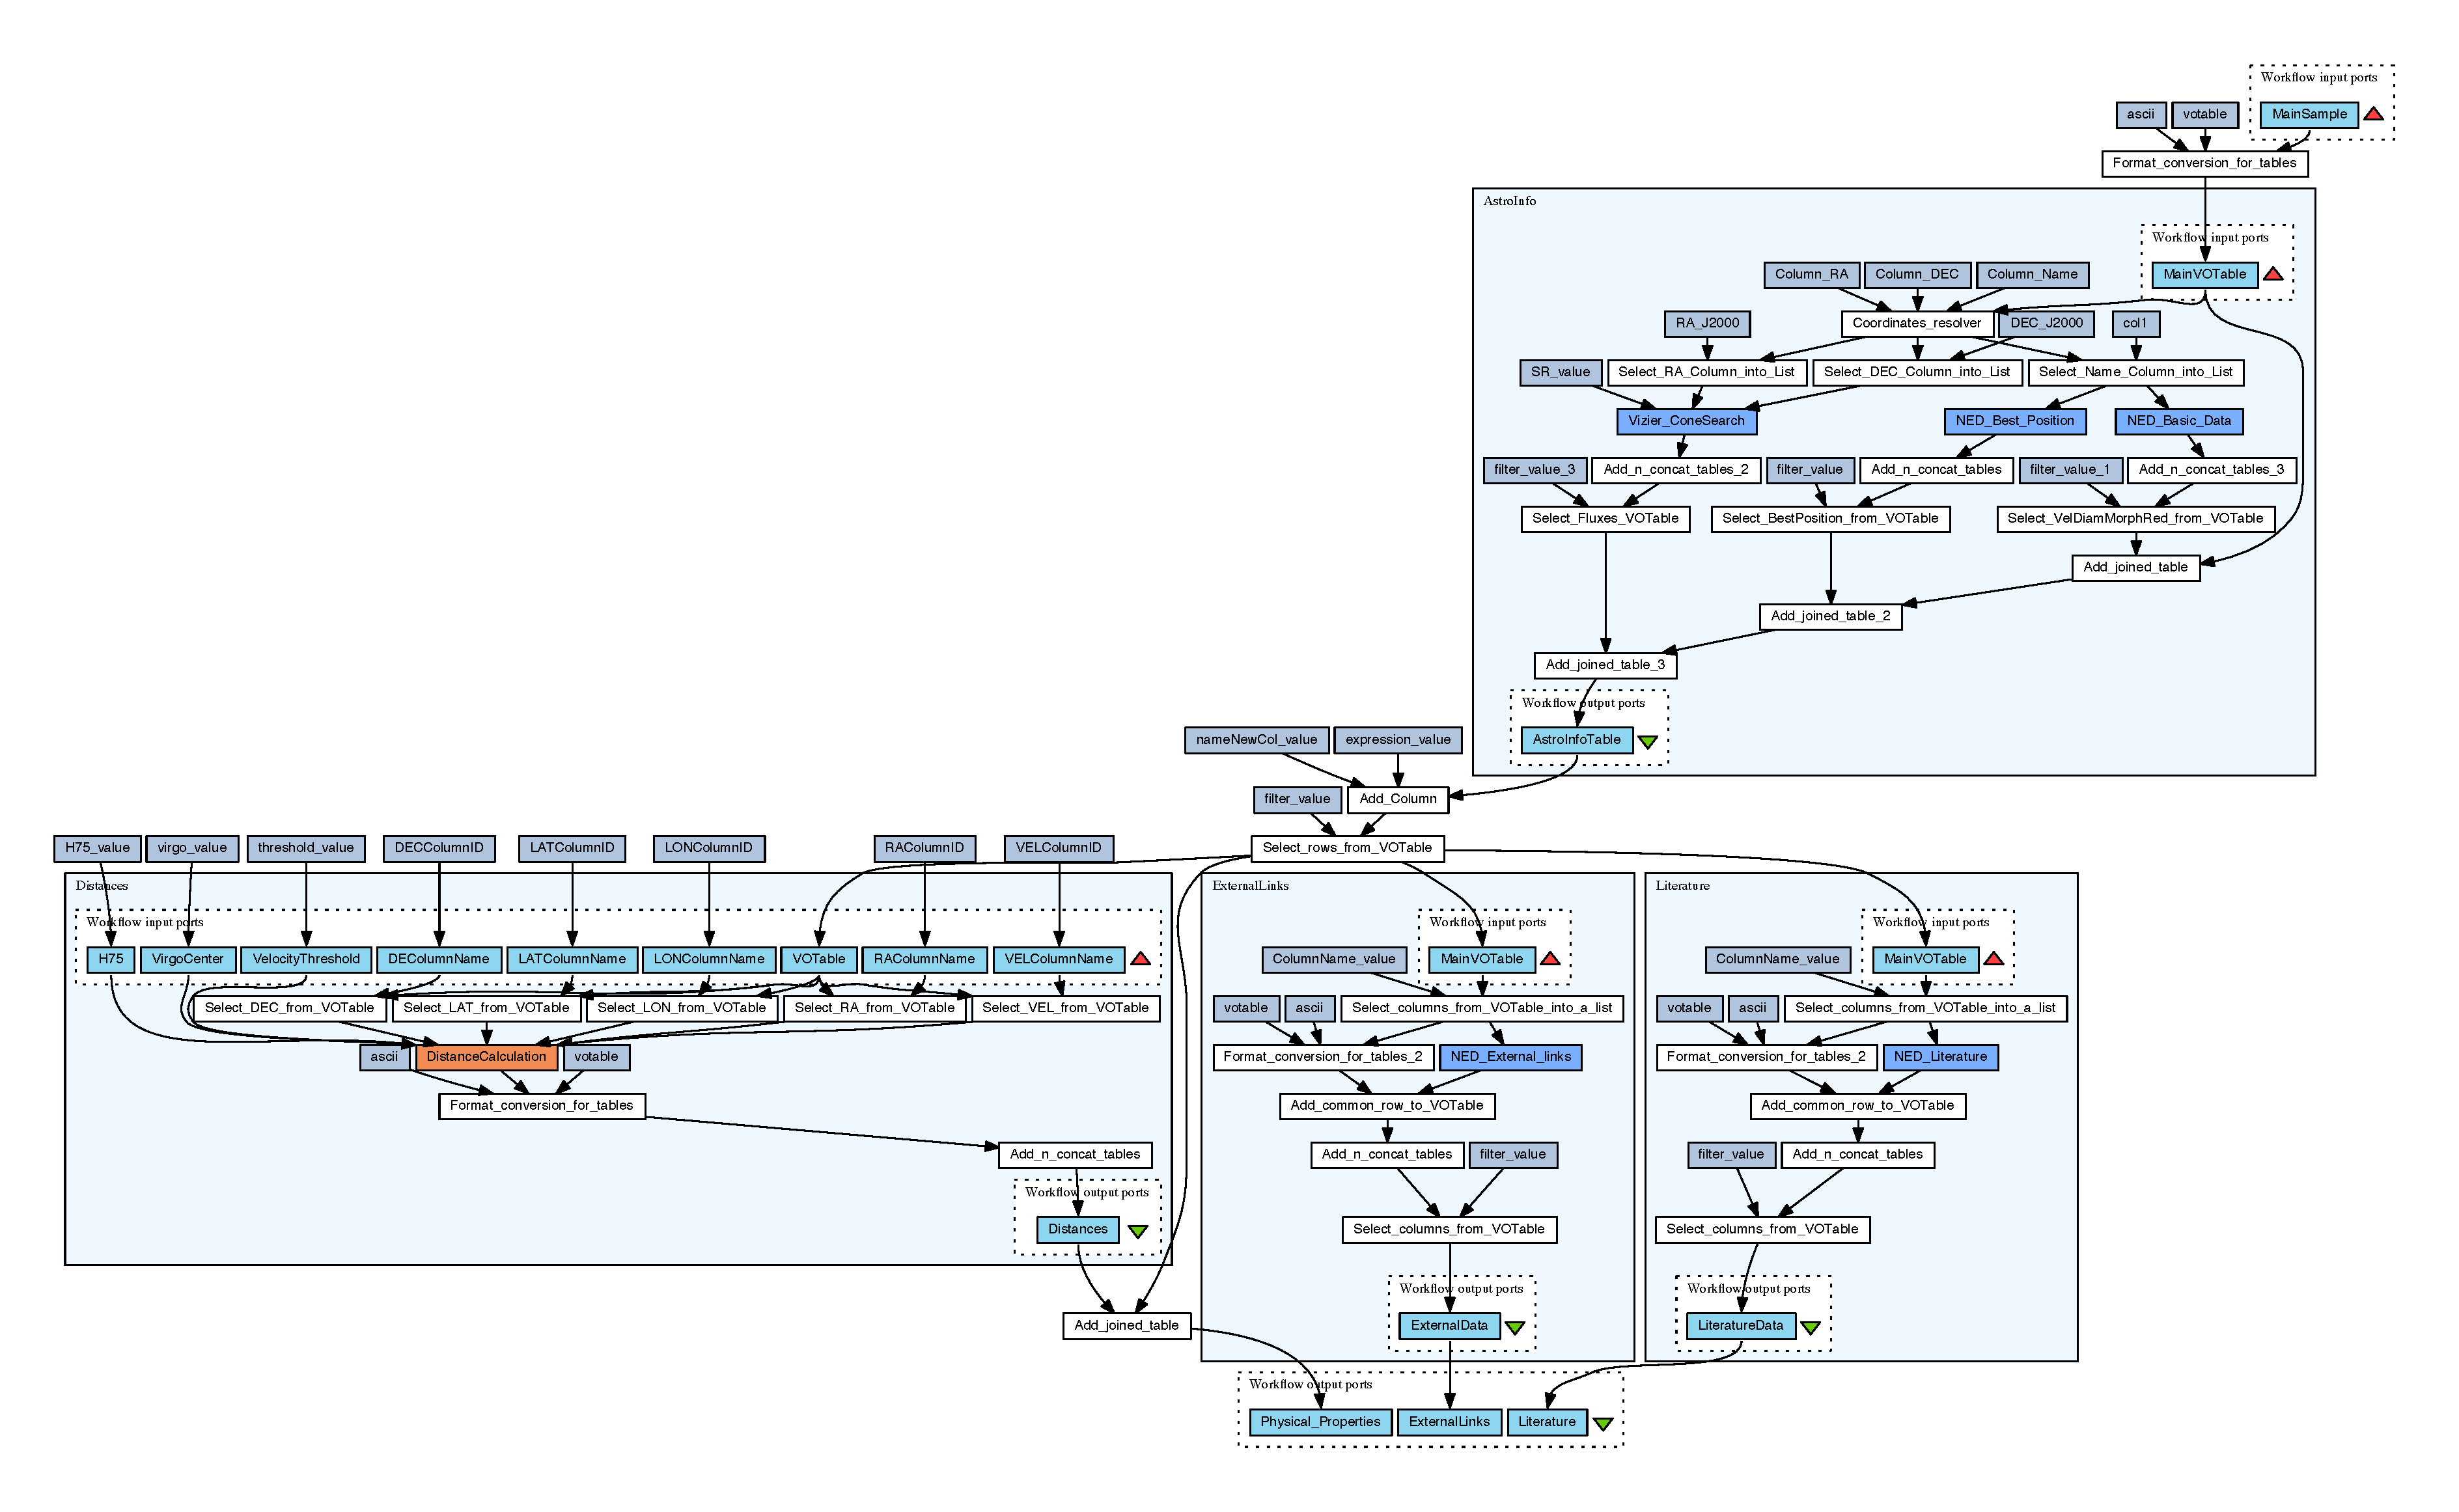
\includegraphics[width=17cm]{WfDiagram.pdf}
\caption{Diagram of AstroTaverna workflow for the example use case described in Sect.~\ref{Usecase}.}
\label{fig:WfDiagram}
\end{figure*}

In this section we illustrate the use of the AstroTaverna plugin with a specific use case consisting on a workflow needing functionalities for VO data gathering, manipulation, transformation and inspection. From an initial sample of galaxy names, we retrieve some of their properties from VO archives and other data services, calculate others based on the previous ones, and complement them with associated bibliography data and links to others related external catalogs.

In this use case we will assumme that this information will be used as the basis for preparing lists of targets for different observational proposals, performing e.g. filtering by positions of galaxies on the sky, size, brightness, etc. The workflow would be re-executed in further occassions in order to provide up-to-date information when needed to prepare a new target list, and possibily slightly modified according to specific needs for different proposals. 

The whole workflow is composed of four different blocks (nested workflows), according to their distinctive roles and actions performed, as seen in Fig.~\ref{fig:WfDiagram}, and it is \hrefnote{http://www.myexperiment.org/workflows/3566}{publicly accessible} through the myExperiment portal. Starting from a list of object names in one ASCII file, the workflow builds up three different VOTables: \textit{Object Properties, Bibliography} and \textit{External Links}.

In a first step it queries, using the name of each galaxy as input, two different data access web services provided by \hrefnote{http://ned.ipac.caltech.edu/}{NASA/IPAC Extragalactic Database (NED)} archive~\citep{Mazzarella2008}.

The following web services provide information for the \textit{Object Properties} VOTable.

\begin{minipage}[h]{0.99\columnwidth}
  \small \vspace{\baselineskip}
  \noindent Service Short Name: NED\_basic\_posn\\
  Service Id: \url{ivo://NED/Basic\_Position\_Data\_For\_Object}\\
  Service Output VOTable Fields:
  \begin{itemize}
	  \item Right Ascension in degrees. (Equatorial J2000.0)
	  \item Declination in degrees. (Equatorial J2000.0)
	  \item Right Ascension in sexagesimal degrees. (Equatorial J2000.0)
	  \item Declination in sexagesimal units. (Equatorial J2000.0)
	  \item Longitude in decimal degrees. (Ecliptic J2000.0)
	  \item Latitude in degrees. (Ecliptic J2000.0)
	  \item Longitude in decimal degrees. (Galactic)
	  \item Latitude in degrees. (Galactic)
	  \item Longitude in decimal degrees. (Super Galactic)
	  \item Latitude in degrees. (Super Galactic)
  \end{itemize}
\end{minipage}

\begin{figure}
\centering 
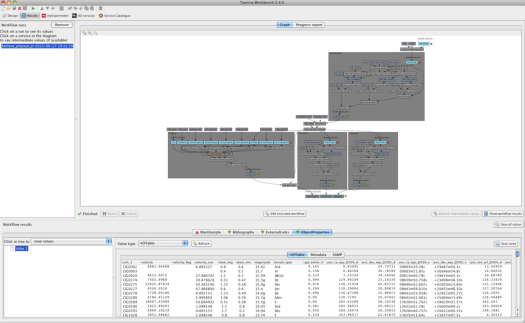
\includegraphics[width=0.99\columnwidth]{WfExec.pdf}
\caption{
Execution of AstroTaverna workflow and rendering of the tabular results for the example use case described in Sect.~\ref{Usecase}.
}
\label{fig:WfExec}
\end{figure}

\begin{minipage}[h]{0.99\columnwidth}
  \small \vspace{\baselineskip}
  \noindent Service Short Name: NED\_basic\\
Service Id: \url{ivo://NED/Basic\_Data\_For\_Object}\\
Service Output VOTable Fields:
\begin{itemize}
\item The heliocentric radial velocity in km/sec.
\item Quality flag for heliocentric radial velocity.
\item Velocity's mean error when known.
\item Major diameter in arcminutes.
\item Minor diameter in arcminutes.
\item Optical magnitude.
\item The morphological type.
\item The Galactic reddening E(B-V), in magnitudes.
\end{itemize}
\vspace{\baselineskip}
\end{minipage}

The workflow makes use of the \textit{VOTable format conversion} AstroTaverna service for making ASCII to VOTable conversion, as well as format conversion for datavalues using STILTS expressions on the \textit{Add column to a VOTable} services. It also queries a specific Vizier ConeSearch service to retrieve data from a published catalog (J/A+A/545/A15). The output VOTable fields retrieved from this catalog are:

\begin{minipage}[h]{0.99\columnwidth}
  \small \vspace{\baselineskip}
  \noindent 
\begin{itemize}
\item Flux density in Ks-band. 
\item Error in the flux density in Ks-band.
\item Log of the luminosity in Ks-band.
\item Error in the log of luminosity in Ks-band.
\end{itemize}
\vspace{\baselineskip}
\end{minipage}

All the previously enumerated fields conform the \textit{Object Properties} VOTable, which is then filtered according to observational and instrumental criteria: e.g. selecting those galaxies with declination greater than twenty degrees and those with observed angular diameter lower than two arc minutes. 

The next step is the calculation of the distance to the selected galaxies, based on their heliocentric radial velocities and sky positions related to the center of Virgo cluster. The workflow executes a Python script as from the command line using the aforementioned parameters as input values. The script is registered and configured in the free-text box of the \textit{Tool} service that is provided by Taverna Workbench. The calculated distances are added to the \textit{Object Properties} VOTable. 

Finally, there are other data access web services provided by NED archive that are queried, in order to complement the sample with related information from bibliography and associated external catalogs. 

The information for the \textit{Bibliography} VOTable is provided by the following web service:

\begin{minipage}[h]{0.9\columnwidth}
  \small \vspace{\baselineskip}
\noindent Service Short Name: NED\_search\_notes\\
Service Id: \url{ivo://ned.ipac/Notes\_By\_Object\_Name}\\
Service Output VOTable Fields:
\begin{itemize}
\item Object Name.
\item The NED 19-digit Bibliographic Reference code (year, journal, volume number, page number, and the initial of the first author's last name).
\item A Note transcribed as faithfully as possible from the catalog or paper.
\end{itemize}
\vspace{\baselineskip}
\end{minipage}

\begin{samepage}
The following web service provides the information for the \textit{External Links} VOTable.

\begin{minipage}[h]{0.9\columnwidth}
  \small \vspace{\baselineskip}
\noindent Service Short Name: NED\_external\\
Service Id: \url{ivo://NED/Basic\_External\_Links\_by\_object\_name}\\
Service Output VOTable Fields:
\begin{itemize}
\item Object Name.
\item NED's link to related on-line astronomical services that are specific to the survey or catalog associated with the NED name.
\item URL address of related on-line astronomical service.
\end{itemize}
\vspace{\baselineskip}
\end{minipage}
\end{samepage}


\section{Results and discussion}
\label{ResultsAndDiscussion}

The AstroTaverna plugin opens a window to astronomy archives by enabling easy design and execution of VO services-based workflows. These strongly rely on the very basic foundation of the Virtual Observatory: public data access, data interoperability and minimized network transfers with lightweight metadata. AstroTaverna workflows also benefit from seamless connectivity with the ecosystem of local SAMP-enabled VO Apps. All these concepts are key in the future development of digital science in Astronomy, where we are already facing the advent of a plethora of astronomical public archives, and transfer network latency is more than an issue. 

Because of the exposed capalities to improve readability and reproducibility of automated tasks, we think workflows could nicely complement the scarce narratives produced in the classic documentation process. Taverna Workbench allows detailed inspection of the different workflow elements, like free text descriptions provided in the services of the workflow and input/output values for any intermediate parameters involved in one particular execution of the workflow or any other previous one.

Transitioning the experimental protocol from manually interacting with graphical user interfaces into a more automated digital flow has made us notice the potential impact of workflows as \textit{living tutorials}, explicitly exposing how to take advantage of existing rich infrastructure of data and services provided by the Virtual Observatory. This is especially relevant with automated execution of Aladin macros and scripts in GUI mode. Scientists may visualize the actions performed by the workflows as they progress in their executions, allowing them to practice self-learning by example, which expedites training and avoids reinvention.  

In this sense, a collection of 29 elemental workflows showcasing the potential of AstroTaverna (workflow snippets) has been developed and published in the myExperiment portal with the name of \hrefnote{http://www.myexperiment.org/packs/420}{\label{starterpack}AstroTaverna Starter Pack}, in order to provide potential users of AstroTaverna a set of small workflows carefully designed to perform very specific actions. These kind of workflows can be considered as \hrefnote{http://www.taverna.org.uk/developers/work-in-progress/components/}{workflow components}, designed to be mixed and nested into larger workflows to perform a particular analysis. 

Digital libraries of workflows could increase the visibility of the scientific outcome, hence its discovery, re-use and a more efficient exploitation of present astronomical archives, computational infrastructures and observational facilities~\citep{Ruiz2012}. Astronomy is a collaborative science, and it has also become highly specialized, as many other disciplines. Sharing, preservation, discovery and a much simplified access to resources in the composition of scientific workflows will enable astronomers to greatly benefit from each other’s highly specialized knowhow, pushing them to share and publish not only results and data, but also processes and methodologies.

Going into more technical considerations, by developing AstroTaverna as a user downloadable plugin, loosely coupled with Taverna Workbench, we can more quickly iterate and add additional capabilities as separated independent developments. In particular, given the dependency of AstroTaverna on the STILTS framework, we can use updated versions of it, bringing bug fixes and new features. By creating the AstroTaverna plugin, we enable the VO as a core building block for Taverna Workbench.

The AstroTaverna plugin was presented in several IVOA Interop conferences in Sao Paolo, Heidelberg and Madrid, as well as in the 8\textsuperscript{th} VO France Workflow Working Group Meeting held in Paris-Meudon Observatory. AstroTaverna has been advertised in \hrefnote{http://www.ivoa.net/newsletter/009/}{Issue 009 of IVOA Newsletter} and through the IVOA general mailing list, together with several video tutorials. These videos may be found in \hrefnote{http://amiga.iaa.es/p/290-astrotaverna.htm}{AMIGA Group website} together with general information and \hrefnote{http://amiga.iaa.es/p/312-astrotools.htm}{documentation} for the AstroTaverna plugin, also present in \hrefnote{http://www.taverna.org.uk/documentation/taverna-plugins/taverna-2-x-plugins/}{Taverna Plugins} website and in the specific \hrefnote{http://wf4ever.github.io/astrotaverna/}{AstroTaverna website}. The source code has been published in Astrophysics Source Code Library~\citep[ASCL; see][]{Garrido2013}, and can be publicly accessed at the \hrefnote{https://github.com/wf4ever/astrotaverna}{GitHub} open source hosting service. Additionally a \hrefnote{http://smtp.iaa.es/mailman/listinfo/astrotaverna-users}{support mailing list} (\textit{astrotaverna-users@iaa.es}) has been created for the AstroTaverna community. 

This work has triggered the interest of VAMDC and ER-Flow EU FP7 funded projects in order to broaden the users community of AstroTaverna and study potential collaborations for developments in the field of workflows. Moreover, AstroTaverna plugin and AstroTaverna Starter Pack have been included recently at the core of specific \hrefnote{http://www.taverna.org.uk/download/workbench/2-5/astronomy/}{Astronomy edition} of the Command Line Tool and the Taverna Workbench 2.5 release, together with project specific plugins from VAMDC and HELIO-VO projects. In addition, a strategy for dissemination and community engagement is being set up with the Spanish Virtual Observatory, where specific use cases are being migrated to AstroTaverna workflows. 

At the moment of writing these lines, the latest version of the AstroTaverna plugin is 1.10. New versions of the plugin are periodically released, not just with bug-fixes, but implementing additional capabilities (e.g. additions of new local services, improvements on VOTable rendering and on the VO Services discovery GUI). We plan to add support for discovery and execution of Table Access Protocol~\citep[TAP;][]{Dowler2010}, handle potential multiple endpoints for a VO service in the discovery process, as well as the possibility to execute AstroTaverna workflows in the Taverna Server. We have explored the possibilities of adding a richer Python support through Jython, but the lack of a pure-python Numpy has precluded that possibility. The orchestration of external services in workflows would greatly benefit from the adoption of web services interoperability standards. In this context, the PDL~\citep[Parameter Description Language;][]{Zwolf2013} has been approved as an IVOA Recomendation in order to deal with web services interoperability in the VO. Next versions of the AstroTaverna plugin will provide a client for PDL self-described services, allowing data input validation before service invocation, providing service metadata description, and services interoperability in the design process of workflows. 

\section{Conclusions}
\label{Conclusions}

We have presented AstroTaverna, a plugin for Taverna Workbench 2.x that provides the means to build astronomy web services-based workflows upon VO services discovery and VOTable efficient manipulation. It integrates SAMP-enabled VO Apps, as well as the possibility to execute Aladin scripts and macros. The plugin is easy to install for any user and operating system, installation instructions may be found in the
AstroTaverna Website\textsuperscript{\ref{website}}. The plugin has been illustrated with a specific use case that considers a workflow making use of local services for VO data gathering, manipulation, transformation and inspection.

AstroTaverna  enables astronomers to capture, in a digital reproducible workflow, the experimental protocol and provenance information otherwise lost in procedural steps manually performed in GUIs of VO Apps. A collection of workflow snippets has been produced with the name of AstroTaverna Starter Pack\textsuperscript{\ref{starterpack}} in order to encourage self-learning by example and avoid reinvention.

Future work considers support for discovery and execution of TAP services, provide a client for PDL self-described services that will allow data input validation before service invocation, handle potential multiple endpoints for a VO service in the discovery process, and the possibility to execute AstroTaverna workflows in the Taverna Server.

\section{Acknowledgements}
\label{Acknowledgements}
We would like to explicitely acknowledge the priceless contribution of Taverna developer Stian Soiland-Reyes, from the School of Computer Science at the University of Manchester, technical software architect and researcher in myGrid project. 

AstroTaverna has been developed in the framework of the \hrefnote{http://www.wf4ever-project.org/}{Wf4Ever Project} 270129 funded under EU FP7 Digital Libraries and Digital Preservation (ICT-2009.4.1), which leverages workflow technology in order to preserve the scientific methodology, facilitating the reuse and exchange of digital knowledge, and to enable the inspection of the reproducibility of scientific investigation results.

Part of the improvements are being undertaken in the framework of \hrefnote{http://amiga.iaa.es/p/294-open-science-canube.htm}{CANUBE Project} CEI2013-P-14, an Open Science project granted by the Second Call for Proposals of the \hrefnote{http://biotic.ugr.es/en/}{Bio-TIC Campus of International Excellence} of the University of Granada, in Spain.

This work has been also supported by grant AYA2011-30491-C02-01, co-financed by MICINN and FEDER funds, and the Junta de Andalucía (Spain) grants P08-FQM-4205 and TIC-114.


%% The Appendices part is started with the command \appendix;
%% appendix sections are then done as normal sections
%% \appendix

%% \section{}
%% \label{}

%% References
%%
%% Following citation commands can be used in the body text:
%%
%%  \citet{key}  ==>>  Jones et al. (1990)
%%  \citep{key}  ==>>  (Jones et al., 1990)
%%
%% Multiple citations as normal:
%% \citep{key1,key2}         ==>> (Jones et al., 1990; Smith, 1989)
%%                            or  (Jones et al., 1990, 1991)
%%                            or  (Jones et al., 1990a,b)
%% \cite{key} is the equivalent of \citet{key} in author-year mode
%%
%% Full author lists may be forced with \citet* or \citep*, e.g.
%%   \citep*{key}            ==>> (Jones, Baker, and Williams, 1990)
%%
%% Optional notes as:
%%   \citep[chap. 2]{key}    ==>> (Jones et al., 1990, chap. 2)
%%   \citep[e.g.,][]{key}    ==>> (e.g., Jones et al., 1990)
%%   \citep[see][pg. 34]{key}==>> (see Jones et al., 1990, pg. 34)
%%  (Note: in standard LaTeX, only one note is allowed, after the ref.
%%   Here, one note is like the standard, two make pre- and post-notes.)
%%
%%   \citealt{key}          ==>> Jones et al. 1990
%%   \citealt*{key}         ==>> Jones, Baker, and Williams 1990
%%   \citealp{key}          ==>> Jones et al., 1990
%%   \citealp*{key}         ==>> Jones, Baker, and Williams, 1990
%%
%% Additional citation possibilities
%%   \citeauthor{key}       ==>> Jones et al.
%%   \citeauthor*{key}      ==>> Jones, Baker, and Williams
%%   \citeyear{key}         ==>> 1990
%%   \citeyearpar{key}      ==>> (1990)
%%   \citetext{priv. comm.} ==>> (priv. comm.)
%%   \citenum{key}          ==>> 11 [non-superscripted]
%% Note: full author lists depends on whether the bib style supports them;
%%       if not, the abbreviated list is printed even when full requested.
%%
%% For names like della Robbia at the start of a sentence, use
%%   \Citet{dRob98}         ==>> Della Robbia (1998)
%%   \Citep{dRob98}         ==>> (Della Robbia, 1998)
%%   \Citeauthor{dRob98}    ==>> Della Robbia


%% References with bibTeX database:

\bibliographystyle{elsarticle-harv}
\bibliography{Workflows}

%% Authors are advised to submit their bibtex database files. They are
%% requested to list a bibtex style file in the manuscript if they do
%% not want to use elsarticle-harv.bst.

%% References without bibTeX database:

% \begin{thebibliography}{00}

%% \bibitem must have one of the following forms:
%%   \bibitem[Jones et al.(1990)]{key}...
%%   \bibitem[Jones et al.(1990)Jones, Baker, and Williams]{key}...
%%   \bibitem[Jones et al., 1990]{key}...
%%   \bibitem[\protect\citeauthoryear{Jones, Baker, and Williams}{Jones
%%       et al.}{1990}]{key}...
%%   \bibitem[\protect\citeauthoryear{Jones et al.}{1990}]{key}...
%%   \bibitem[\protect\astroncite{Jones et al.}{1990}]{key}...
%%   \bibitem[\protect\citename{Jones et al., }1990]{key}...
%%   \harvarditem[Jones et al.]{Jones, Baker, and Williams}{1990}{key}...
%%

% \bibitem[ ()]{}

% \end{thebibliography}

\end{document}

%%
%% End of file `AstroTaverna.tex'.
